\chapter{Especificación del Problema}
\label{chap:especificacion_problema}

\section{Antecedentes y soluciones existentes} % (fold)
\label{sec:antecedentes_y_soluciones_existentes}

A continuación se presentan algunas de las soluciones existentes que apuntan a resolver problemas similares al de esta memoria.

\subsection{LittleSis y Poderopedia} % (fold)
\label{sub:littlesis_y_poderopedia}

% * que es littlesis
% * screenshot de littlesis
% * por que no cumplo el objetivo de la memoria con littlesis
\textbf{LittleSis}, pequeña hermana en oposición al gran hermano (Big Brother), es una plataforma estadounidense que contiene una base de datos libre de relaciones de \emph{quien conoce a quien} en el mundo de las grandes empresas y políticas de ese país. Todo esto con el fin de entregar información a la gente sobre qué posibles conflictos de intereses pueden tener los políticos que toman las decisiones en el país.

\begin{figure}[H]
  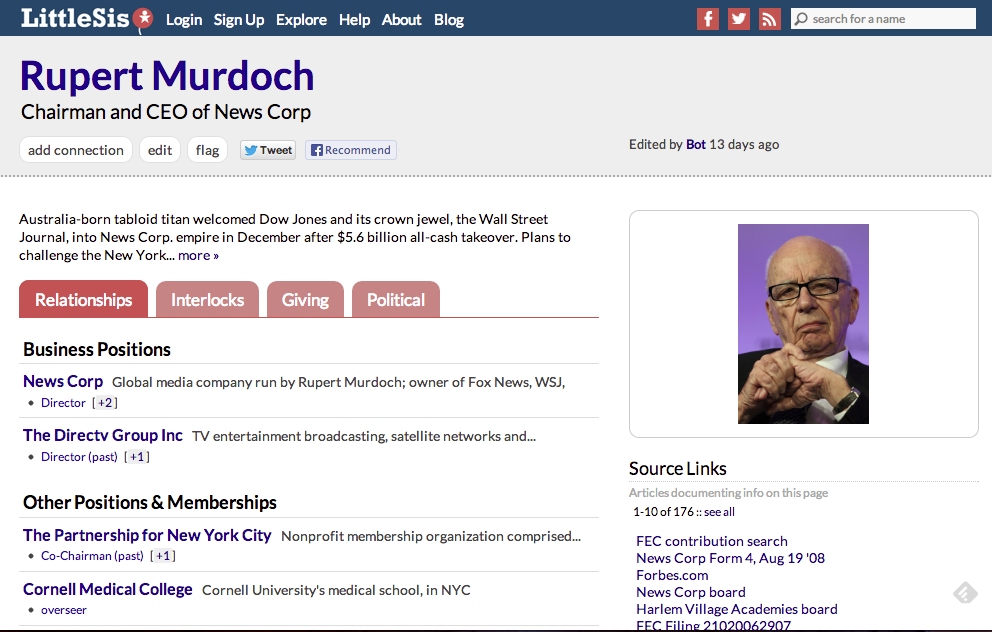
\includegraphics[width=1.0\textwidth]{images/littlesis.png}
  \caption[Interfaz de LittleSis, Rupert Murdoch]{\emph{Interfaz de LittleSis, Rupert Murdoch}. un ejemplo de como littlesis almacena la información de las personas y el tipo de personas presentes en littleSis.}
  \label{ejemplo_littlesis}
\end{figure}

La idea detrás de LittleSis de entregar el poder de la información a la gente es muy buena desde su punto de vista de análisis de estructuras sociales económicas y políticas. Sin embargo, no cubre el problema que trata resolver esta memoria, debido a que si bien las personas pueden complementar esta información, esto se hace de una manera centralizada, además de que no se puede agregar información asociada a otro tipos de redes sociales, como por ejemplo: la red de panaderos de un país, ya que no está dentro del objetivo y alcance de LittleSis, sin mencionar que esta idea está enfocada en Estados Unidos.\\

\textbf{Poderopedia} es el clon chileno de LittleSis, una plataforma centralizada por la cual se expone información sobre las redes de poder e influencias en el ambiente económico, social y político chileno, en donde nuevamente el objetivo es enfocarse en las personas de los más altos cargos empresariales y políticos en Chile.\\

\begin{figure}[H]
  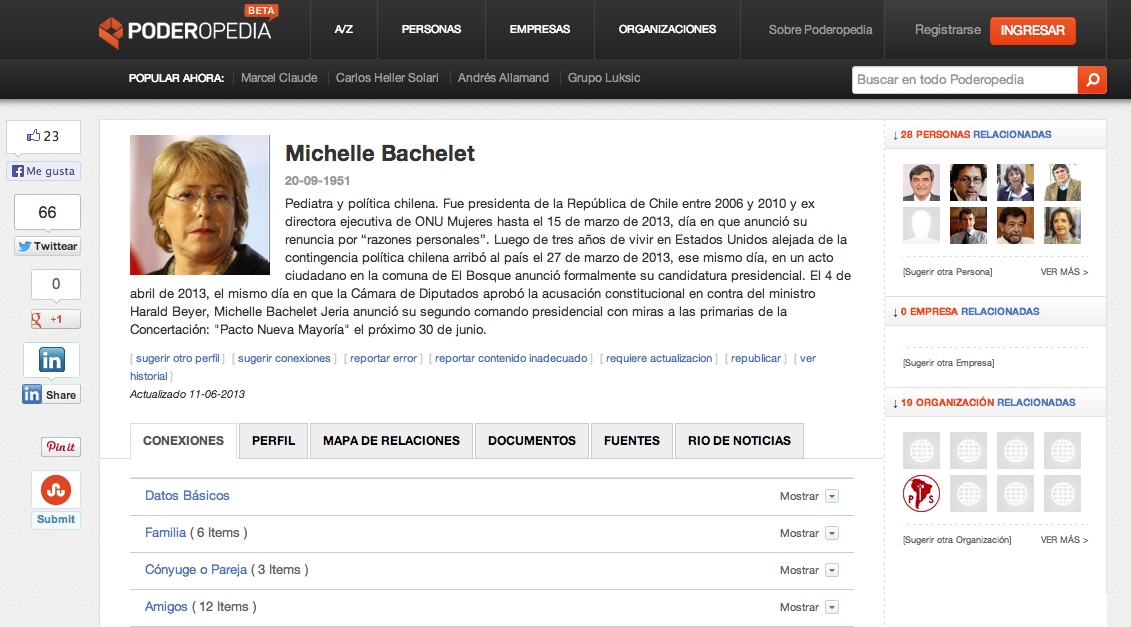
\includegraphics[width=1.0\textwidth]{images/poderopedia.png}
  \caption[Interfaz de Poderopedia, Michelle Bachelet]{\emph{Interfaz de Poderopedia, Michelle Bachelet}. un ejemplo de como poderopedia almacena la información de las personas y el tipo de personas presentes en esta plataforma.}
  \label{ejemplo_poderopedia}
\end{figure}

\begin{figure}[H]
  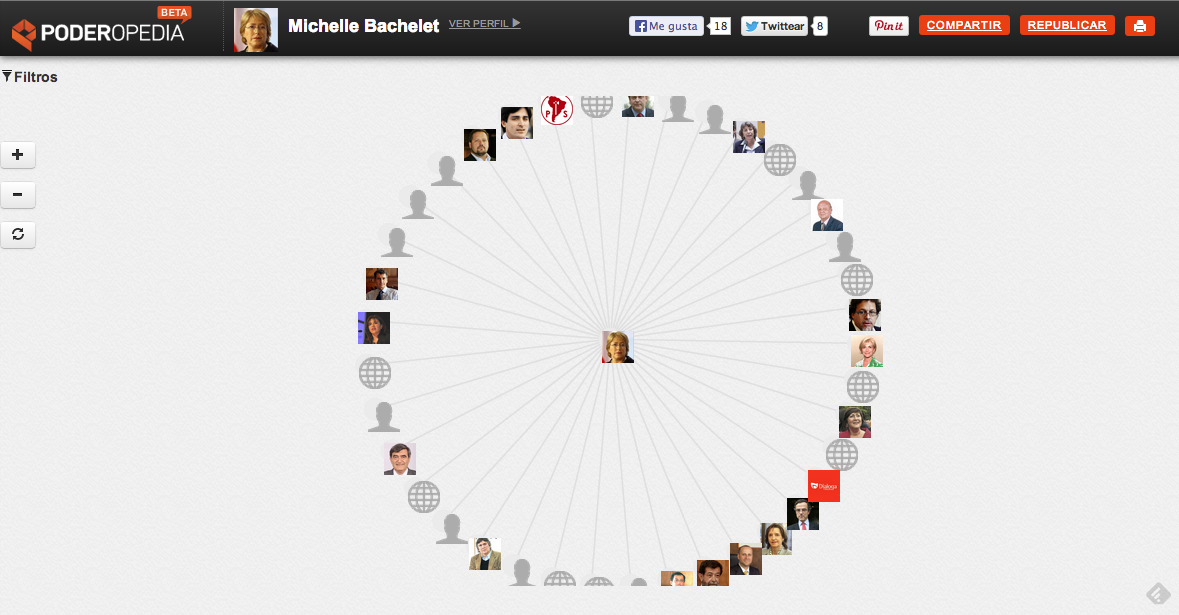
\includegraphics[width=1.0\textwidth]{images/grafo_poderopedia.png}
  \caption[Interfaz de Grafo de Poderopedia, Michelle Bachelet]{\emph{Interfaz de Grafo de Poderopedia, Michelle Bachelet}. Poderopedia tiene una opción de visualización de grafo al rededor de una persona.}
  \label{ejemplo_grafo_poderopedia}
\end{figure}

De la misma forma de LittleSis, las desventajas de Poderopedia en relación al problema que se desea resolver en esta memoria, van por el lado de que su foco es exclusivamente la gente con poder político y económico del país, que además es centralizada, que su visualización de grafo no entrega información real de las estructuras sociales y no es fácilmente manipulable.\\

Ambos LittleSis y Poderopedia son excelentes herramientas, pero su objetivo difiere de lo que se desea resolver en esta memoria, a pesar de que la idea básica es la misma, exponer información sobre estructuras sociales.

% subsection littlesis_y_poderopedia (end)

\subsection{Memoria Manuel Bahamonde} % (fold)
\label{sub:memoria_manuel_bahamonde}

% TODO ver que se refiere claudio con XXXXXX
Un intento de resolver este problema fue desarrollado por el alumno del DCC Manuel Bahamonde, quien hizo su trabajo de memoria titulado: \emph{Aplicación para la creación y administración de redes sociales} \cite{memoriamanuel} el año 2009, memoria también guiada por el profesor Claudio Gutiérrez. Entonces, se gestó la idea de este trabajo de memoria, como una forma de mejorar lo XXXXXX anteriormente por Manuel, aprovechando los avances tecnológicos y experiencias con el modelamiento de redes sociales y la web semántica.\\

La aplicación desarrollada en Java por Manuel, permite al usuario descargar un ejecutable y usarlo tanto en Windows, Linux o Mac, la cual permite crear redes sociales en forma de grafo, creando actores y sus relaciones respectivas, asociándolos a familias y pudiendo exportar la información de las redes sociales en formato para la utilización del software de análsis de redes sociales, pajek\cite{pajek}.

\begin{figure}[H]
  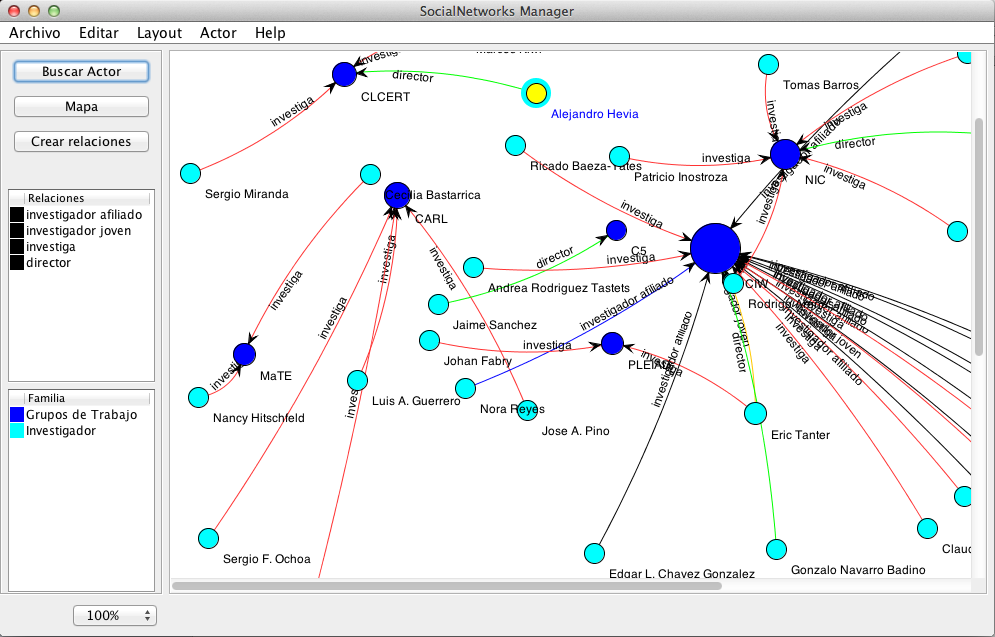
\includegraphics[width=1.0\textwidth]{images/memoria_manuel.png}
  \caption[Interfaz SocialNetworks Manager]{\emph{Interfaz SocialNetworks Manager}. La aplicación creada por el alumno Manuel Bahamonde con el objetivo de modelar redes sociales como aproximación incial al problema de esta memoria.}
  \label{memoria_manuel}
\end{figure}

El trabajo de Manuel ayudó como experiencia para acercarse más a una solución para el modelamiento de redes sociales y con el conocimiento actual del tema, es necesario hacer modificaciones a lo que hizo Manuel, resolviendo algunos problemas extras, como:

  \begin{enumerate}
    \item El formato de almacenamiento de las redes sociales, no permite una interoperabilidad con otras aplicaciones fuera de pajek\cite{pajek}, en especial con las tecnologías de la web semántica.
    \item Las relaciones entre actores sólo pueden ser 2 actores a la vez, no hay posibilidad de crear n-relaciones, o relaciones entre $n$ actores.
    \item Esta aplicación no permite complementar la información de una red social uniéndola con otra.
    \item No se puede agregar atributos a los actores y relaciones.
    \item Necesita que el usuario de la aplicación tenga instalado Java en su equipo.
    \item No se puede acceder a la información del usuario desde cualquier computador.
    \item La interfaz podría ser mejor en términos de usabilidad
  \end{enumerate}

% subsection memoria_manuel_bahamonde (end)

\subsection{Otras Alternativas} % (fold)
\label{sub:otras_alternativas}

% * que otras referencias de soluciones similares tengo?

Dentro de las otras opciones disponibles al tema de esta memoria, se tiene algunos softwares de creación y visualización de grafos, como por ejemplo yED\cite{yed} u OnmniGraffle\cite{omnigraffle}. Este tipo de soluciones sólo genera los grafos de forma visual, sin tener los datos estructurados de la red para poder ser analizados posteriormente por otra aplicación, además de que no ayudan con la creación efectiva de redes sociales, pues no poseen un esquema concreto de redes sociales por ser herramientas de visualización multipropósito.\\

Otras herramientas existentes de la rama de análisis de redes sociales son por ejemplo Gruff\cite{gruff} que es una herramienta de visualización de la base de datos AllegroGraph\cite{allegrograph}, la cual no posee las características que permiten crear redes sociales en forma estructurada, en base a un modelo estándar que se sepa que funciona, como el modelo SNM de Mauro San Martín\cite{tesismauro}. Por otro lado, se encuentra Graph\cite{graph}, que es una herramienta de visualización de grafos genéricos, que en este caso comparte los problemas de Gruff, para el manejo de redes sociales, un caso específico de grafo.\\

Por lo tanto dentro de las alternativas disponibles investigadas, entre otras, las características distintivas claves de este trabajo de memoria es la capacidad de unir redes sociales, el uso de un modelo estándar para redes sociales y la generación de datos RDF con la herramienta.

% subsection otras_alternativas (end)

% section antecedentes_y_soluciones_existentes (end)

%   
% #### Otras referencias
% 
% * que otras referencias de soluciones similares tengo?

% ### 3.2 Relevancia del problema
% 
% * el problema es relevante de tomar pues se le entrega a las personas una herramienta que les permite guardar datos de
% redes sociales en forma interactiva y gráfica.
% * permite que las personas puedan complementar su información con la información de otras personas
% * permite la generación de información compatible con la web semántica por parte de personas con conocimientos básicos
% de computación
\section{Relevancia del Problema} % (fold)
\label{sec:relevancia_del_problema}

El problema es relevante de resolver, debido a que se está entregando una herramienta que le permitiría a personas que no tengan conocimientos avanzados de computación, almacenar redes sociales en forma gráfica interactivamente.\\

Además estas redes sociales anteriormente creadas, se pueden complementar uniéndolas con otras redes sociales creadas por otros usuarios de la aplicación, aprovechando el conocimiento de más personas sobre estructuras sociales determinadas.\\

Otro aspecto clave de resolver este problema con este tipo de aplicación corresponde a que los datos generados por sus usuarios son compatibles con los formatos y tecnologías pertenecientes a la web semántica, por lo cual esta información puede ser relacionada con otras fuentes de conocimiento posteriormente.

% section relevancia_del_problema (end)


% ### 3.3 Usuarios Objetivo
% 
% * quienes son mis usuarios objetivo
\section{Usuarios Objetivo} % (fold)
\label{sec:usuarios_objetivo}

La herramienta que se desarrollará para esta memoria está enfocada principalmente en personas en cuya profesión requiera el estudio de diversos tipos de redes sociales, las cuales pueden encontrarse en campos como: sociología, biología, historia, negocios etc. Es decir personas con un conocimiento básico de redes sociales y el estudio de estas, aplicadas a algún campo en particular.

% section usuarios_objetivo (end)

\section{Requisitos de la Aplicación} % (fold)
\label{sec:requisitos_de_la_aplicacion}

% ### 3.4 Requisitos / Criterios de Aceptación
% 
% se especifica en todo el detalle de los requisitos **(del informe del E)**
% 
% *Es una visión más funcional de los requisitos que se necesitan cumplir*
% 
% Se necesita un sistema que me permita crear y editar redes sociales y:
% * crear, editar y borrar actores
% * crear, edirar y borrar relaciones n-árias entre esos actores
% * que me permita agregar, editar y borrar atributos de actores y relaciones
% * que pueda unir redes sociales
% * que pueda exportar mis redes sociales en formato RDF
% * que pueda importar mis redes en formato RDF
% 
% En términos de requisitos de calidad se necesita:
% 
% * que la interfaz sea fácil de usar
% * que la aplicación sea de fácil instalación

Una vez especificado el contexto del problema a resolver, se exponen los requisitos funcionales y de calidad de la aplicación que busca resolver las necesidades planteadas, escritas como requisitos que puedan ser usados posteriormente como criterios de aceptación de la aplicación del trabajo de memoria, un sistema de creación y manejo de redes sociales:

\subsection{Requisitos Funcionales} % (fold)
\label{sub:requisitos_funcionales}

\begin{enumerate}
  \item Creación de usuario para identificación dentro del sistema.
  \item Creación, edición y eliminación de redes sociales y sus componentes.
  \item Dentro de las redes sociales, crear, editar y eliminar actores y sus atributos.
  \item Dentro de las redes sociales, crear, editar y eliminar relaciones n-árias (entre $n$ actores) y sus atributos.
  \item Exportar los datos de una red social en formato RDF.
  \item Importar/Cargar datos de una red social en formato RDF.
  \item Unir redes sociales.
\end{enumerate}

% subsection requisitos_funcionales (end)

\subsection{Requisitos de Calidad} % (fold)
\label{sub:requisitos_de_calidad}

\begin{enumerate}
  \item Una aplicación fácil de usar.
  \item Mantener la transparencia con el manejo de información, que las personas sean dueñas de sus datos.
  \item Una aplicación de fácil instalación.
\end{enumerate}

% subsection requisitos_de_calidad (end)

% section requisitos_de_la_aplicación (end)